
\documentclass[12pt,a4paper]{report}

% --------------------------------------------------
% Packages
% --------------------------------------------------

\usepackage[utf8]{inputenc}
\usepackage[T1]{fontenc}
\usepackage[french]{babel}
\usepackage{lmodern}

\usepackage{geometry}
\geometry{
    left=2.5cm,
    right=2.5cm,
    top=2.5cm,
    bottom=2.5cm
}

\usepackage{graphicx}
\usepackage{float}
\usepackage{booktabs}
\usepackage{array}
\usepackage{amsmath,amssymb}
\usepackage{siunitx}
\usepackage{xcolor}
\usepackage{caption}
\usepackage{subcaption}
\usepackage{hyperref}
\usepackage{setspace}

\hypersetup{
    colorlinks=true,
    linkcolor=blue,
    urlcolor=blue,
    citecolor=blue
}

\setlength{\parindent}{0.5cm}
\setlength{\parskip}{0.3em}
\onehalfspacing

\usepackage{pgfplots}
\pgfplotsset{compat=1.18}

% --------------------------------------------------
% Informations du rapport
% --------------------------------------------------

\title{
    \textbf{Calibration d'une caméra}\\[0.4cm]
    \large Estimation des paramètres intrinsèques,
    de la distorsion et de la pose
}

\author{
    Fallou Diouf\\
    Master 2 -- Vision et Machine Intelligente\\
    Université Paris Cité
}

\date{Année universitaire 2026--2027}

% --------------------------------------------------
% Début du document
% --------------------------------------------------

\begin{document}

\maketitle

\tableofcontents
\clearpage

% ==================================================
\chapter{Introduction}
% ==================================================

La calibration d'une caméra est une étape fondamentale
en vision par ordinateur. Elle consiste à déterminer
les paramètres géométriques qui caractérisent le
système de formation des images, notamment les
paramètres intrinsèques de la caméra ainsi que les
paramètres décrivant les distorsions optiques de
l'objectif.

Ces paramètres permettent d'établir une relation
géométrique entre les points d'une scène tridimensionnelle
et leurs projections dans le plan image. Ils sont
notamment nécessaires pour des applications telles que
la reconstruction 3D, la localisation d'une caméra
et la mesure géométrique à partir d'images.

L'objectif de ce travail est de réaliser la calibration
d'une caméra de smartphone à partir de plusieurs
photographies d'un damier. À partir des images acquises,
nous cherchons à détecter les points caractéristiques
du damier, estimer les paramètres intrinsèques de la
caméra, corriger les distorsions optiques et déterminer
la pose de la caméra pour chaque vue.

L'évaluation de la calibration repose notamment sur
l'analyse des erreurs de reprojection, qui permettent
de mesurer l'écart entre les positions observées des
points dans les images et leurs positions calculées
à partir du modèle géométrique estimé.

% ==================================================
\chapter{Acquisition et constitution du dataset}
% ==================================================

\section{Matériel utilisé}

L'acquisition des images a été réalisée à l'aide de
la caméra arrière principale d'un smartphone
\textbf{Samsung Galaxy A14 4G}.

Les photographies ont été prises avec le zoom
principal (1$\times$), sans utiliser de zoom numérique.
Le damier utilisé comme cible de calibration a été
affiché sur l'écran d'un ordinateur Mac à partir
d'un fichier PDF.

Le tableau suivant présente les principales
caractéristiques du dispositif expérimental.

\begin{table}[H]
    \centering
    \caption{Caractéristiques du dispositif d'acquisition.}
    \label{tab:acquisition}
    \begin{tabular}{ll}
        \toprule
        \textbf{Élément} & \textbf{Caractéristique} \\
        \midrule
        Caméra & Samsung Galaxy A14 4G \\
        Module utilisé & Caméra arrière principale \\
        Zoom & 1$\times$ \\
        Résolution initiale & $4080 \times 3060$ pixels \\
        Focale indiquée dans les EXIF & \SI{4.0}{mm} \\
        Ouverture & $f/1.8$ \\
        Cible & Damier affiché sur écran \\
        Taille physique d'une case & \SI{15}{mm} \\
        \bottomrule
    \end{tabular}
\end{table}

La taille physique des cases du damier a été vérifiée
à l'aide d'une règle. La longueur du côté d'une case
est de \SI{1.5}{cm}, soit \SI{15}{mm}. Cette mesure
est utilisée pour construire les coordonnées
tridimensionnelles des points du damier.

\section{Acquisition des images}

Une série de 19 photographies a été acquise le
28 octobre 2026. Pendant l'acquisition, la position
et l'orientation du smartphone ont été modifiées
par rapport au damier afin d'obtenir différentes
vues de la cible.

Cette variation des points de vue permet de disposer
d'observations géométriques complémentaires. Elle
est importante pour estimer les paramètres de la
caméra à partir de plusieurs configurations du damier.

Les images originales ont été enregistrées au format
HEIC avec une résolution de
$4080 \times 3060$ pixels.

\section{Prétraitement des images}

Avant la détection des points du damier, les images
ont subi plusieurs opérations de préparation :

\begin{enumerate}
    \item Conversion des fichiers HEIC au format PNG ;
    \item Normalisation de l'orientation des images
    afin d'obtenir une disposition cohérente ;
    \item Redimensionnement des images de
    $4080 \times 3060$ à
    $2040 \times 1530$ pixels ;
    \item Organisation des images préparées dans
    un répertoire dédié au traitement.
\end{enumerate}

Le redimensionnement a été effectué en conservant
le rapport d'aspect des images. Il permet de réduire
le coût de calcul tout en conservant une résolution
suffisante pour détecter les coins du damier.

\section{Sélection du dataset final}

Bien que 19 photographies aient été initialement
acquises, 18 images ont été retenues pour la
calibration finale et l'estimation des poses.

Une première analyse des erreurs de reprojection
a permis d'identifier une vue présentant un écart
plus important que les autres. Cette image,
\texttt{20261028\_155639.png}, n'a pas été retenue
dans le jeu de données final.

Le dataset utilisé pour les traitements finaux
contient donc 18 images de résolution
$2040 \times 1530$ pixels.

\begin{table}[H]
    \centering
    \caption{Bilan de la constitution du dataset.}
    \label{tab:dataset}
    \begin{tabular}{lr}
        \toprule
        \textbf{Description} & \textbf{Nombre} \\
        \midrule
        Images initialement acquises & 19 \\
        Images retenues & 18 \\
        Images écartées & 1 \\
        Résolution des images traitées & $2040 \times 1530$ \\
        \bottomrule
    \end{tabular}
\end{table}

\textbf{Remarque :} la cible étant affichée sur un écran,
la taille physique des cases a été vérifiée directement
sur l'affichage utilisé lors de l'acquisition. La
précision de cette mesure constitue un élément à
prendre en compte dans l'interprétation des
paramètres métriques estimés.


% ==================================================
\chapter{Détection des points caractéristiques du damier}
% ==================================================

\section{Configuration du damier}

Le damier constitue la cible géométrique utilisée
pour la calibration. Il est composé d'une alternance
de cases noires et blanches. Les intersections entre
les cases constituent des points caractéristiques
dont les positions peuvent être détectées dans les
images.

La configuration utilisée comporte 9 colonnes et
6 lignes de coins intérieurs, soit un total de :

\begin{equation}
    N = 9 \times 6 = 54 \text{ points}.
\end{equation}

Chaque point détecté dans une image est associé à
un point correspondant dans le repère tridimensionnel
du damier. Comme la cible est plane, les coordonnées
de ces points sont définies dans le plan $Z=0$.

En prenant comme origine le premier coin intérieur
du damier et en considérant une taille de case
$a = \SI{15}{mm}$, les coordonnées des points
du damier sont définies par :

\begin{equation}
    \mathbf{P}_{i,j} =
    \begin{bmatrix}
        i\,a \\
        j\,a \\
        0
    \end{bmatrix},
    \qquad
    \begin{cases}
        i = 0,\ldots,8,\\
        j = 0,\ldots,5.
    \end{cases}
\end{equation}

Cette représentation fournit un ensemble de
54 points tridimensionnels de référence.

\section{Détection des coins dans les images}

La détection des coins du damier a été réalisée
avec la fonction
\texttt{cv2.findChessboardCorners()} de la
bibliothèque OpenCV.

Cette fonction recherche automatiquement les
intersections internes du damier en utilisant
la configuration attendue, définie par le nombre
de coins horizontaux et verticaux.

Dans notre implémentation, la configuration est
définie par :

\begin{verbatim}
CHECKERBOARD = (9, 6)
\end{verbatim}

Pour chaque image, la détection est effectuée
sur une version en niveaux de gris. Cette
transformation permet de travailler sur
l'intensité lumineuse sans dépendre directement
des informations de couleur.

La détection fournit les coordonnées des coins
dans le plan image, exprimées en pixels.
Ces coordonnées constituent les observations
bidimensionnelles associées aux points 3D
du damier.

\section{Raffinement subpixel des coordonnées}

Les coordonnées initialement obtenues par la
détection peuvent être affinées afin d'améliorer
la précision de localisation des coins.

Pour cela, nous avons utilisé la fonction
\texttt{cv2.cornerSubPix()} d'OpenCV. Cette
fonction ajuste la position de chaque coin
dans son voisinage afin d'obtenir une estimation
plus précise que la localisation initiale
à la précision du pixel.

Le raffinement a été réalisé avec les paramètres
suivants :

\begin{itemize}
    \item Taille de la fenêtre de recherche :
    $11 \times 11$ pixels ;
    \item Critère d'arrêt : combinaison d'un
    nombre maximal de 30 itérations et d'une
    précision de convergence de $10^{-3}$.
\end{itemize}

Le critère d'arrêt utilisé peut être représenté
par :

\begin{equation}
    \text{critère} =
    \left(
        \text{EPS} + \text{MAX\_ITER},
        30,
        10^{-3}
    \right).
\end{equation}

Le raffinement subpixel permet ainsi d'obtenir
des coordonnées flottantes pour les points
caractéristiques, ce qui est important pour
la précision des étapes de calibration et
d'estimation de pose.

\section{Résultats de la détection}

La détection a été exécutée sur les 19 images
initialement acquises. Les 54 coins intérieurs
ont été détectés et affinés pour chacune de ces
images.

Après la sélection du jeu de données final,
18 images ont été conservées pour les étapes
suivantes. Chaque image retenue fournit donc
54 correspondances entre les points du damier
dans le repère tridimensionnel et leurs positions
observées dans le plan image.

Le nombre total de points image utilisés pour
la calibration finale est ainsi :

\begin{equation}
    N_{\mathrm{total}} = 18 \times 54 = 972.
\end{equation}

\begin{table}[H]
    \centering
    \caption{Bilan de la détection des points caractéristiques.}
    \label{tab:detection}
    \begin{tabular}{lr}
        \toprule
        \textbf{Indicateur} & \textbf{Résultat} \\
        \midrule
        Nombre de coins intérieurs & 54 \\
        Configuration du damier & $9 \times 6$ \\
        Images analysées & 19 \\
        Images retenues pour la suite & 18 \\
        Points détectés par image retenue & 54 \\
        Correspondances image finales & 972 \\
        \bottomrule
    \end{tabular}
\end{table}

Les coordonnées raffinées ont été enregistrées
dans un fichier au format NumPy afin d'être
réutilisées lors de la calibration intrinsèque
et de l'estimation des poses.

\begin{verbatim}
results/image_points_original_2040.npz
\end{verbatim}

Ce fichier contient notamment les coordonnées
des points détectés, les noms des images
correspondantes ainsi que les dimensions
des images traitées.

\begin{figure}[H]
     \centering
     \includegraphics[width=0.8\textwidth]
     {/Users/falloudiouf/Desktop/SequenceVideo/camera_calibration/results/corners_original_2040/20261028_155614.png}
     \caption{Détection et raffinement des 54 coins
     intérieurs du damier dans une image.}
     \label{fig:detection-coins}
\end{figure}


\chapter{Calibration de la caméra}

\section{Principe de la calibration}

La calibration consiste à estimer les paramètres intrinsèques de la caméra ainsi que ses coefficients de distorsion optique. Elle repose sur les correspondances entre les points 3D connus du damier et leurs positions 2D détectées dans les images.

Les points du damier sont définis dans un repère associé à celui-ci. Pour chaque image, leur projection dans le plan image dépend des paramètres intrinsèques de la caméra, des paramètres extrinsèques (rotation et translation) et de la distorsion optique.

La matrice intrinsèque est définie par :

\[
K =
\begin{bmatrix}
f_x & 0 & c_x \\
0 & f_y & c_y \\
0 & 0 & 1
\end{bmatrix}
\]

où :
\begin{itemize}
    \item $f_x$ et $f_y$ représentent les distances focales exprimées en pixels ;
    \item $c_x$ et $c_y$ représentent les coordonnées du point principal ;
    \item les paramètres extrinsèques décrivent la position et l'orientation du damier par rapport à la caméra.
\end{itemize}

Les coefficients de distorsion sont modélisés par le vecteur :

\[
D = (k_1, k_2, p_1, p_2, k_3)
\]

Les coefficients $k_1$, $k_2$ et $k_3$ décrivent la distorsion radiale, tandis que $p_1$ et $p_2$ décrivent la distorsion tangentielle.

\section{Estimation des paramètres}

La calibration a été réalisée avec la fonction \texttt{cv2.calibrateCamera()} de la bibliothèque OpenCV. Les données utilisées sont les coordonnées 3D des 54 coins du damier et leurs coordonnées 2D détectées dans les 18 images retenues.

La taille des images utilisées est de $2040 \times 1530$ pixels. La taille d'un carré du damier est fixée à 15 mm.

La fonction estime simultanément la matrice intrinsèque, les coefficients de distorsion et les paramètres extrinsèques propres à chaque image. L'estimation repose sur la minimisation de l'erreur de reprojection entre les points détectés et leurs positions calculées par le modèle de caméra.

\section{Résultats de la calibration}

La calibration sur les 18 images retenues donne une erreur quadratique moyenne de reprojection de :

\[
\boxed{\mathrm{RMS} = 0{,}2678 \text{ pixel}}
\]

La matrice intrinsèque estimée est :

\[
K =
\begin{bmatrix}
1638{,}6939 & 0 & 1020{,}4124 \\
0 & 1640{,}5535 & 762{,}8702 \\
0 & 0 & 1
\end{bmatrix}
\]

Les coefficients de distorsion obtenus sont :

\[
D =
\begin{bmatrix}
0{,}2061 &
-0{,}6083 &
0{,}000596 &
0{,}000585 &
-0{,}2928
\end{bmatrix}
\]

Les valeurs de $f_x$ et $f_y$ sont proches, ce qui indique que les échelles horizontale et verticale estimées sont similaires. Le point principal estimé se situe à proximité du centre de l'image.

L'erreur RMS représente l'écart global entre les points observés et les points reprojetés par le modèle sur l'ensemble des vues utilisées.

\begin{table}[H]
\centering
\caption{Paramètres estimés lors de la calibration}
\label{tab:parametres-calibration}
\begin{tabular}{lll}
\toprule
\textbf{Paramètre} & \textbf{Valeur} & \textbf{Unité} \\
\midrule
$f_x$ & 1638,6939 & pixel \\
$f_y$ & 1640,5535 & pixel \\
$c_x$ & 1020,4124 & pixel \\
$c_y$ & 762,8702 & pixel \\
$f$ physique & 4,1951 & mm \\
$f$ physique & 0,0041951 & m \\
\midrule
RMS de calibration & 0,2678 & pixel \\
\bottomrule
\end{tabular}
\end{table}


\section{Estimation de la longueur focale physique}

La matrice intrinsèque obtenue lors de la calibration fournit les distances focales
$f_x$ et $f_y$ exprimées en pixels. Cependant, pour caractériser physiquement
l'objectif de la caméra, il est intéressant d'exprimer sa longueur focale en
millimètres ou en mètres.

Pour effectuer cette conversion, nous avons utilisé la fonction
\texttt{cv2.calibrationMatrixValues()} d'OpenCV. Cette fonction exploite la
matrice intrinsèque ainsi que les dimensions physiques du capteur pour calculer
la longueur focale physique et les champs de vision de la caméra.

Les dimensions du capteur utilisées dans notre expérience sont :
\begin{itemize}
    \item Largeur : $5{,}2224$ mm ;
    \item Hauteur : $3{,}9168$ mm.
\end{itemize}

Ces dimensions sont des estimations utilisées pour le calcul et ne constituent
pas des dimensions officielles confirmées par le constructeur.

Les résultats obtenus sont présentés dans le tableau suivant :

\begin{table}[H]
\centering
\caption{Caractéristiques optiques estimées de la caméra}
\label{tab:focale}
\begin{tabular}{lr}
\toprule
\textbf{Caractéristique} & \textbf{Valeur} \\
\midrule
Longueur focale estimée & $4{,}1951$ mm \\
Longueur focale estimée & $0{,}004195$ m \\
Champ de vision horizontal & $63{,}80^\circ$ \\
Champ de vision vertical & $50{,}00^\circ$ \\
Point principal physique & $(2{,}6123\,;\,1{,}9529)$ mm \\
Rapport d'aspect & $1{,}001135$ \\
\midrule
Longueur focale issue des métadonnées EXIF & $4{,}0$ mm \\
\bottomrule
\end{tabular}
\end{table}

La longueur focale estimée par calibration est de $4{,}1951$ mm, soit
$0{,}004195$ m. Cette valeur est proche de celle indiquée dans les métadonnées
EXIF des photographies, qui est de $4{,}0$ mm. L'écart entre les deux valeurs
est d'environ $0{,}1951$ mm, soit $4{,}88\,\%$ par rapport à la valeur EXIF.

Cette comparaison constitue une vérification de cohérence intéressante.
Toutefois, elle doit être interprétée avec prudence, car la conversion en
unités physiques dépend des dimensions du capteur utilisées, qui sont ici
estimées.


\chapter{Estimation des poses de la caméra}

\section{Principe de l'estimation de pose}

Après avoir estimé les paramètres intrinsèques et les coefficients de
distorsion de la caméra, nous avons procédé à l'estimation de sa pose
pour chacune des 18 images retenues.

L'objectif est de déterminer la rotation et la translation entre le
repère associé au damier et le repère de la caméra. Pour cela, nous
avons utilisé la fonction \texttt{cv2.solvePnP()} d'OpenCV.

Cette fonction exploite les correspondances entre les coordonnées 3D
des coins du damier et leurs coordonnées 2D dans l'image, ainsi que
les paramètres intrinsèques et les coefficients de distorsion
précédemment estimés.

La transformation entre un point exprimé dans le repère du damier
et sa position dans le repère caméra s'écrit :

\[
\mathbf{X}_c = R\mathbf{X}_o + \mathbf{t}
\]

où :
\begin{itemize}
    \item $\mathbf{X}_o$ représente les coordonnées 3D du point dans
    le repère du damier ;
    \item $\mathbf{X}_c$ représente ses coordonnées dans le repère
    de la caméra ;
    \item $R$ est la matrice de rotation ;
    \item $\mathbf{t}$ est le vecteur de translation.
\end{itemize}

La matrice de rotation décrit l'orientation relative entre les deux
repères, tandis que le vecteur de translation décrit leur décalage
relatif.

\section{Résultats de l'estimation des poses}

L'estimation a été réalisée indépendamment pour chacune des 18 images.
Pour chaque vue, la fonction \texttt{cv2.solvePnP()} fournit un vecteur
de rotation et un vecteur de translation. Le vecteur de rotation est
ensuite converti en matrice de rotation afin de faciliter
l'interprétation géométrique.

Nous avons également calculé la position du centre de la caméra dans
le repère du damier à partir de la relation :

\[
\mathbf{C} = -R^T\mathbf{t}
\]

Les translations et les positions sont exprimées en millimètres,
puisque les coordonnées 3D du damier ont été construites à partir
d'une taille de carré de 15 mm.

Les poses estimées permettent ainsi de décrire les différentes
positions et orientations de la caméra lors de l'acquisition des
photographies.

\section{Visualisation 3D des poses estimées}

Afin de mieux interpréter les résultats de l'estimation de pose,
nous avons réalisé une représentation tridimensionnelle des
18 positions et orientations de la caméra dans le repère du damier.

Dans cette représentation, le plan noir correspond au plan du
damier, qui constitue le repère de référence. Les points bleus
indiquent les positions des centres des caméras pour les
différentes prises de vue. Les trois axes colorés représentent
l'orientation de chaque caméra : rouge pour l'axe X, vert pour
l'axe Y et bleu pour l'axe Z.

Cette visualisation met en évidence la diversité des positions
et des orientations adoptées par la caméra lors de l'acquisition
des 18 photographies. Les centres des caméras sont situés à
différentes distances du damier et présentent des orientations
variées.

La représentation permet ainsi de vérifier visuellement la
cohérence géométrique des poses estimées et de mieux comprendre
la configuration spatiale utilisée pour la calibration.

\begin{figure}[H]
    \centering
    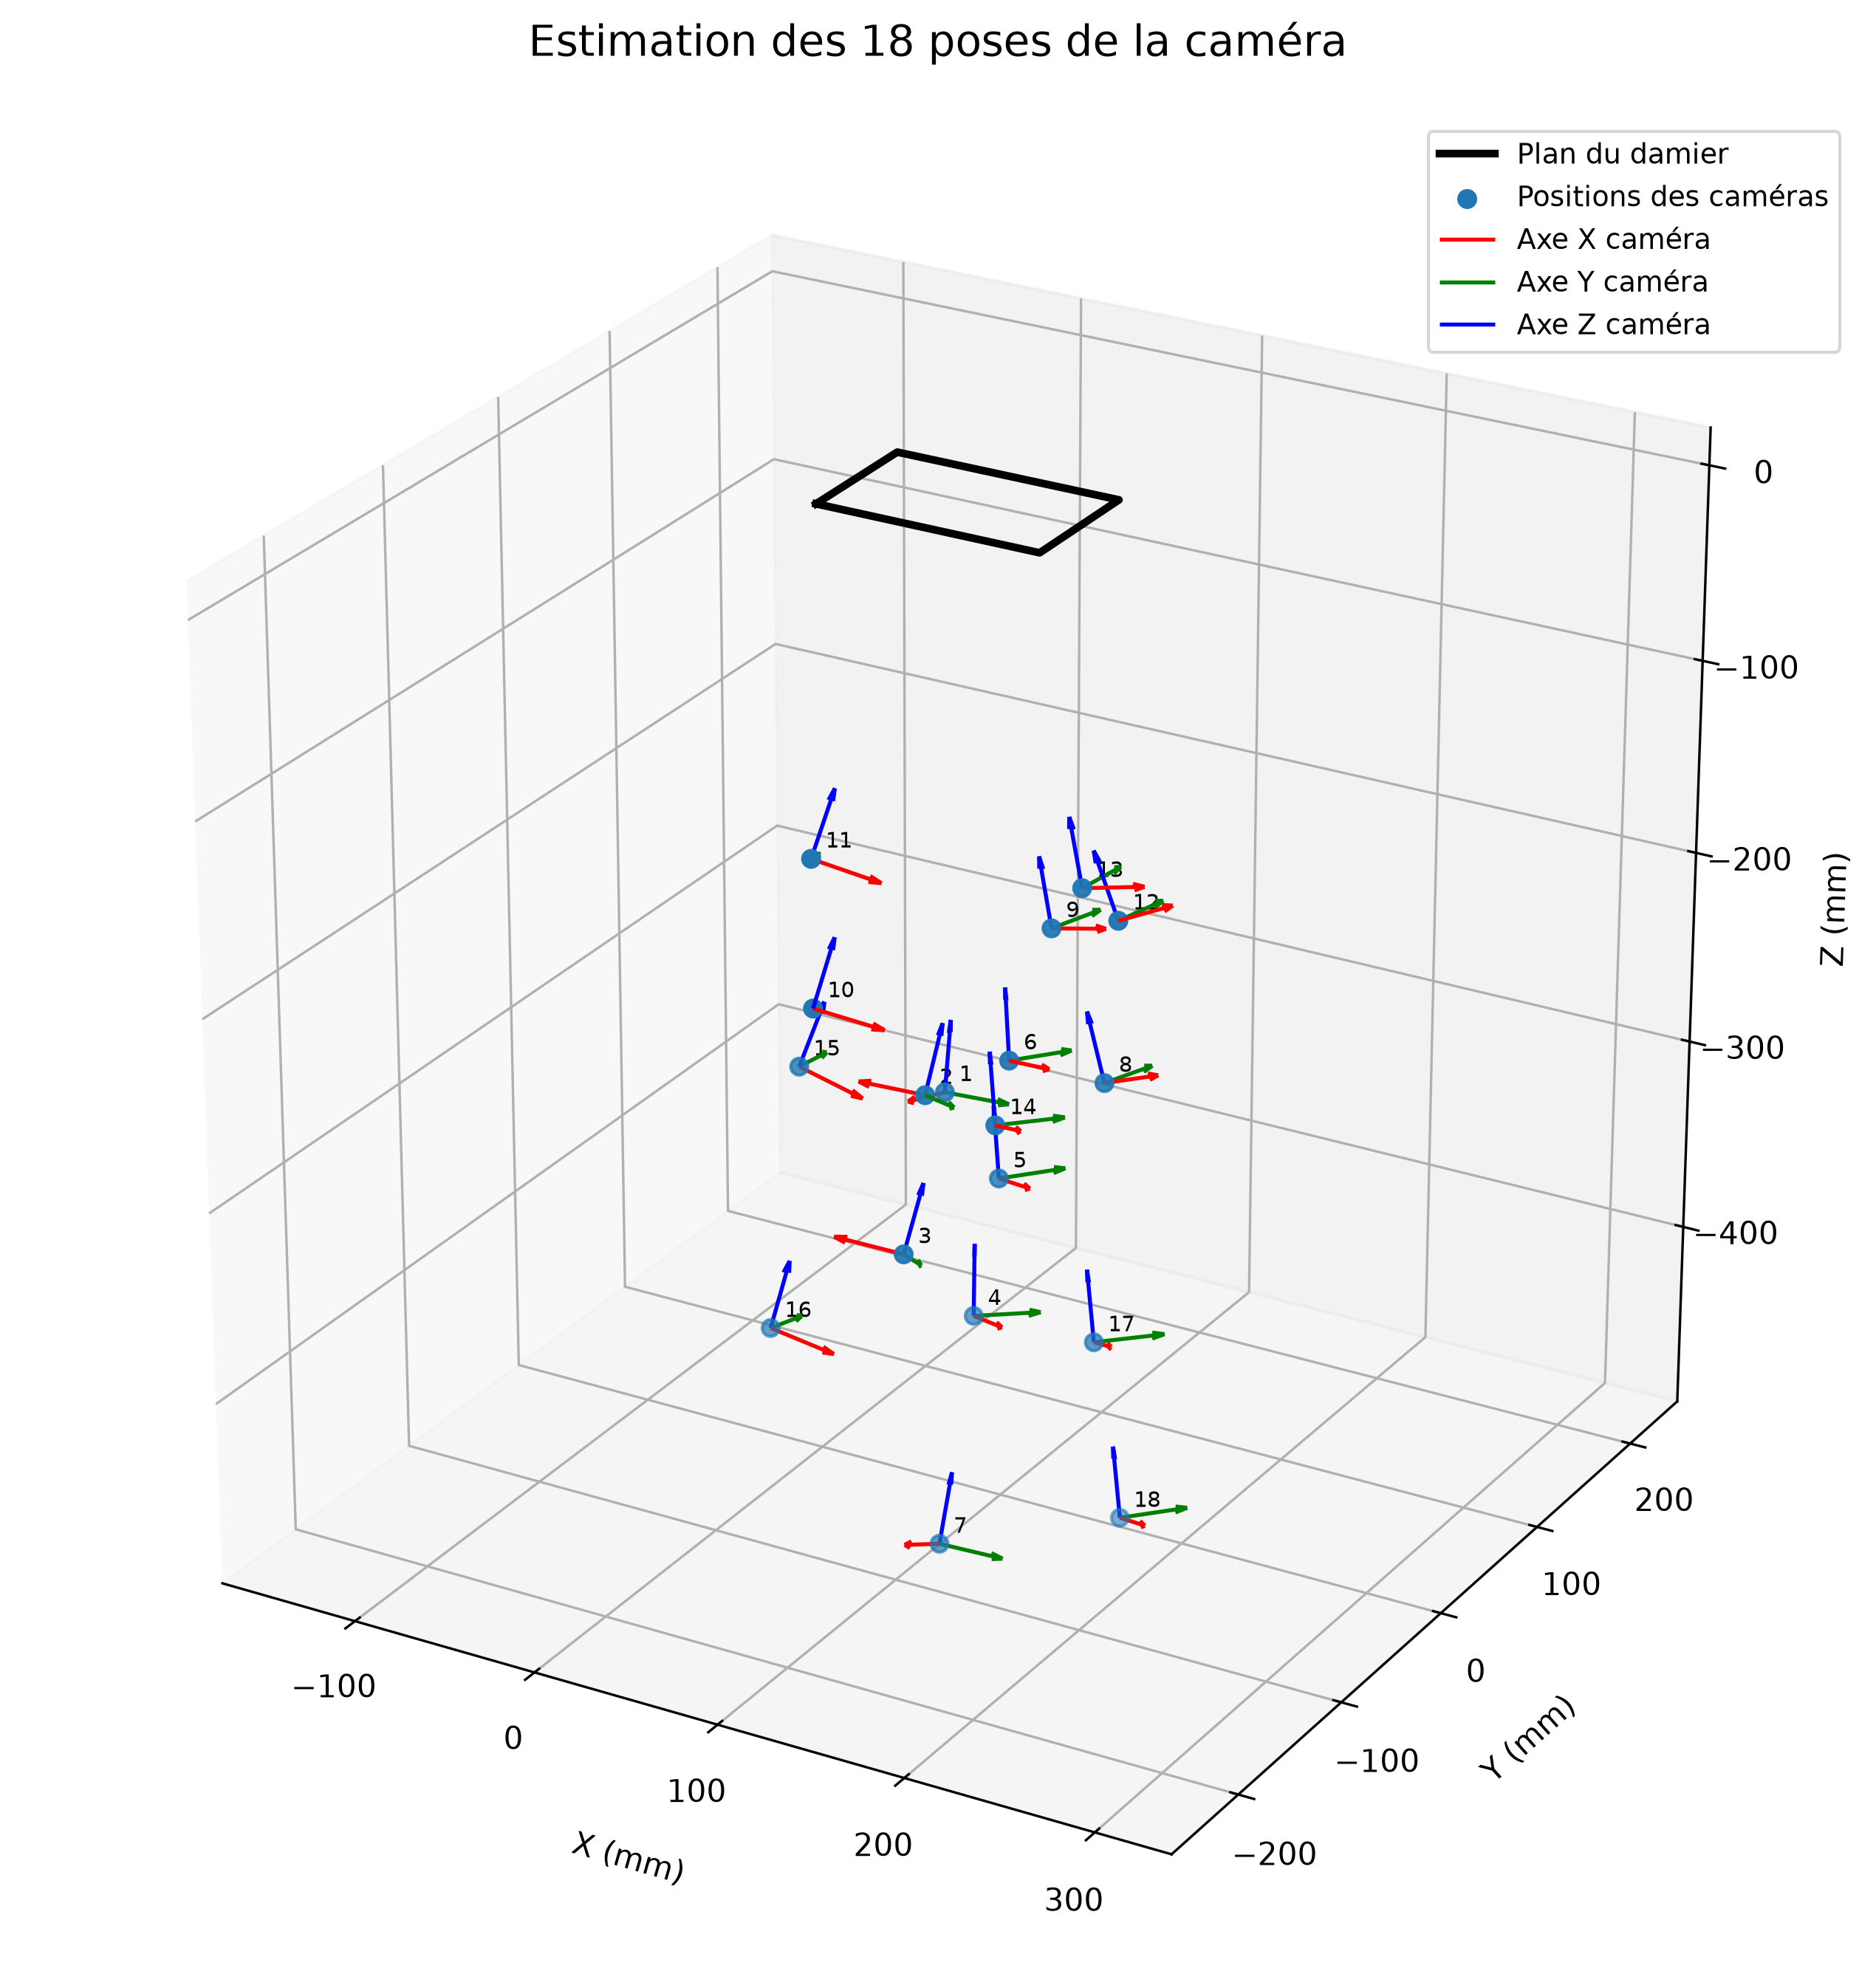
\includegraphics[width=0.85\textwidth]
    {figures/camera_poses_3d.png}
    \caption{Représentation 3D des 18 poses estimées de la caméra
    dans le repère du damier.}
    \label{fig:poses-3d}
\end{figure}

\section{Évaluation par l'erreur de reprojection}

Afin d'évaluer la cohérence des poses estimées, nous avons calculé
l'erreur de reprojection pour chaque image.

Le principe consiste à reprojeter les points 3D du damier dans le
plan image à l'aide des paramètres estimés, puis à comparer leurs
positions projetées aux positions réellement détectées.

Pour un point $i$, l'erreur de reprojection est définie par :

\[
e_i =
\left\|
\mathbf{p}_i^{\mathrm{observé}} -
\mathbf{p}_i^{\mathrm{projeté}}
\right\|_2
\]

où $\mathbf{p}_i^{\mathrm{observé}}$ désigne la position du coin
détecté dans l'image et $\mathbf{p}_i^{\mathrm{projeté}}$ sa position
calculée par le modèle de caméra.

L'évaluation a été réalisée sur les 18 images utilisées pour
l'estimation des poses.

Les résultats globaux obtenus sont les suivants :

\begin{table}[H]
\centering
\caption{Bilan de l'erreur de reprojection sur les 18 images}
\label{tab:erreur-reprojection}
\begin{tabular}{lr}
\toprule
\textbf{Indicateur} & \textbf{Valeur (pixel)} \\
\midrule
Nombre d'images & 18 \\
Erreur moyenne & 0,2146 \\
RMSE moyen par image & 0,2484 \\
Erreur maximale observée & 1,2359 \\
\bottomrule
\end{tabular}
\end{table}

L'erreur moyenne de reprojection est de 0,2146 pixel, tandis que
la moyenne des RMSE calculés individuellement pour chaque image
est de 0,2484 pixel. L'erreur maximale observée parmi les points
reprojetés est de 1,2359 pixel.

Ces résultats indiquent une bonne proximité entre les positions
des coins détectés et celles calculées par le modèle de caméra.
Ils permettent d'évaluer la cohérence géométrique des poses estimées
sur les différentes vues.

\section{Visualisation des reprojections}

Pour visualiser cette évaluation, nous avons représenté les coins
détectés et leurs positions reprojetées sur une même image.

Les points détectés sont représentés par des marqueurs verts,
les points reprojetés par des croix rouges et les segments bleus
illustrent les écarts entre les deux positions.

La figure suivante présente un exemple de cette comparaison pour
l'image \texttt{20261028\_155747.png}.

% À adapter au nom exact du fichier de visualisation.
\begin{figure}[H]
    \centering
    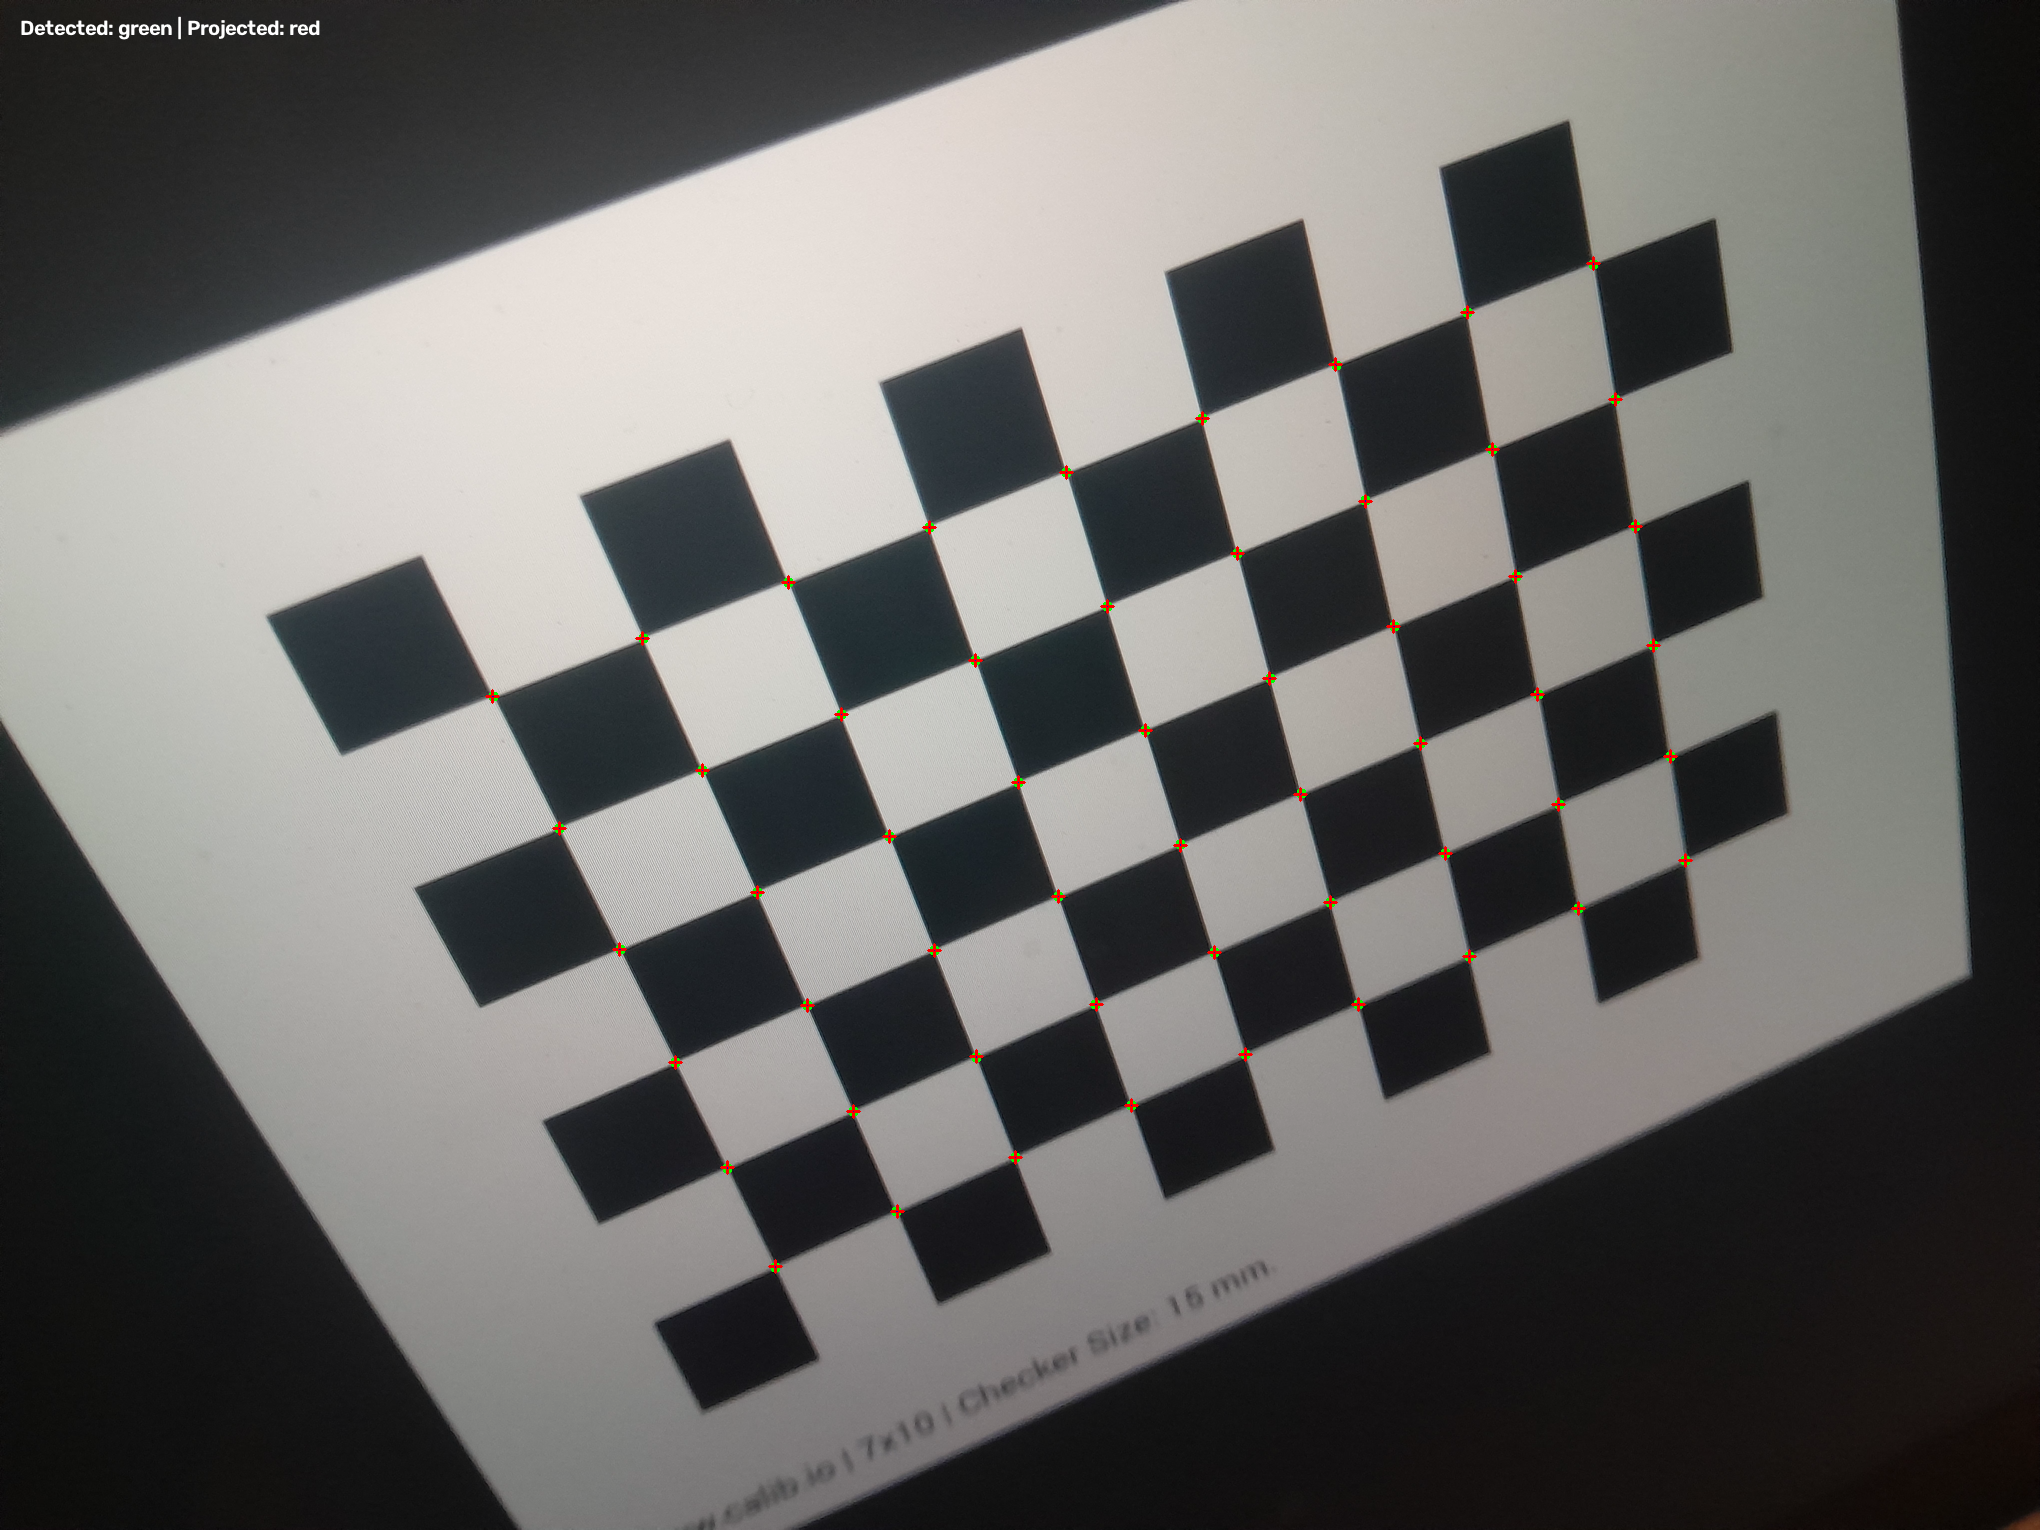
\includegraphics[width=0.85\textwidth]
    {figures/reprojection_visualization.png}
    \caption{Comparaison entre les coins détectés et les points
    reprojetés pour une vue du damier.}
    \label{fig:reprojection}
\end{figure}

On observe que les points reprojetés sont globalement proches des
points détectés. Cette superposition visuelle est cohérente avec
les faibles erreurs de reprojection obtenues numériquement.

\section{Analyse comparative des erreurs par image}

Afin d'étudier la répartition des erreurs de reprojection, nous
avons comparé l'erreur moyenne obtenue pour chacune des
18 images utilisées lors de l'estimation des poses.

La figure~\ref{fig:erreurs-par-image} présente les erreurs
moyennes de reprojection en pixels pour chaque vue.

\begin{figure}[H]
    \centering
    \begin{tikzpicture}
    \begin{axis}[
        ybar,
        width=0.95\textwidth,
        height=7cm,
        bar width=7pt,
        xlabel={Images},
        ylabel={Erreur moyenne (pixels)},
        ymin=0,
        ymax=0.45,
        xtick={1,...,18},
        xticklabels={
            155614,155625,155631,155648,155655,155701,
            155711,155726,155730,155741,155747,155800,
            155807,155819,155825,155831,155836,155841
        },
        x tick label style={rotate=55,anchor=east,font=\small},
        ymajorgrids=true,
        grid style=dashed,
        enlarge x limits=0.03,
    ]
    \addplot coordinates {
        (1,0.1467)
        (2,0.1506)
        (3,0.1077)
        (4,0.1286)
        (5,0.2191)
        (6,0.1935)
        (7,0.2236)
        (8,0.3280)
        (9,0.3262)
        (10,0.1992)
        (11,0.3530)
        (12,0.3991)
        (13,0.2941)
        (14,0.1654)
        (15,0.1444)
        (16,0.1309)
        (17,0.1622)
        (18,0.1900)
    };
    \end{axis}
    \end{tikzpicture}
    \caption{Erreurs moyennes de reprojection obtenues pour
    chacune des 18 images.}
    \label{fig:erreurs-par-image}
\end{figure}

Les erreurs moyennes varient entre 0,1077 et 0,3991 pixel.
L'image \texttt{20261028\_155800.png} présente l'erreur moyenne
la plus élevée, avec 0,3991 pixel, tandis que l'image
\texttt{20261028\_155631.png} présente la plus faible,
avec 0,1077 pixel.

Malgré ces variations entre les différentes vues, les erreurs
moyennes restent inférieures à 0,4 pixel. Cette observation
montre que les résultats de reprojection sont relativement
homogènes sur les 18 images, même si certaines vues présentent
des écarts plus importants que d'autres.

\section{Bilan}

L'estimation des poses a permis de déterminer les positions et
les orientations relatives de la caméra par rapport au damier
pour les 18 images retenues.

La visualisation tridimensionnelle met en évidence la diversité
des points de vue acquis. L'évaluation par reprojection montre
une erreur moyenne de 0,2146 pixel et une moyenne des RMSE
individuels de 0,2484 pixel.

Ces résultats indiquent une bonne cohérence entre les
correspondances observées dans les images et les projections
calculées à partir du modèle de caméra estimé.

\chapter{Correction de la distorsion des images}

\section{Principe de la correction}

Après la calibration de la caméra, nous avons utilisé les paramètres
intrinsèques et les coefficients de distorsion estimés afin de
corriger les déformations géométriques présentes dans les images.

En effet, les objectifs photographiques peuvent introduire des
déformations qui entraînent un écart entre la position réelle d'un
point dans la scène et sa position dans l'image acquise. Ces
déformations sont principalement modélisées par les coefficients
de distorsion radiale et tangentielle estimés lors de la calibration.

La correction consiste à appliquer le modèle inverse de distorsion
afin d'obtenir une image dont la géométrie est plus proche de la
projection idéale du modèle de caméra.

\section{Méthode utilisée}

La correction a été réalisée à l'aide des fonctions OpenCV
\texttt{cv2.getOptimalNewCameraMatrix()} et
\texttt{cv2.undistort()}.

La première fonction permet de calculer une nouvelle matrice
intrinsèque adaptée à la correction et de déterminer une région
d'intérêt (\textit{Region of Interest}, ROI). La seconde applique
la correction à l'image à partir de la matrice intrinsèque,
de la nouvelle matrice et des coefficients de distorsion estimés.

Nous avons utilisé le paramètre $\alpha = 1$ lors du calcul de la
nouvelle matrice intrinsèque. Ce choix permet de conserver
l'ensemble du champ de vision initial, au prix de l'apparition
éventuelle de zones noires dans les bordures de l'image corrigée.

\section{Résultats de la correction}

Les images corrigées ont été obtenues à partir des images
originales redimensionnées à une résolution de
$2040 \times 1530$ pixels.

La comparaison entre les images avant et après correction permet
d'observer l'effet de la compensation de la distorsion optique.
Les bordures peuvent notamment présenter des transformations
géométriques et des zones noires résultant du processus de
correction.

La figure suivante présente un exemple de comparaison entre
une image originale et son équivalent corrigé.

\begin{figure}[H]
    \centering
    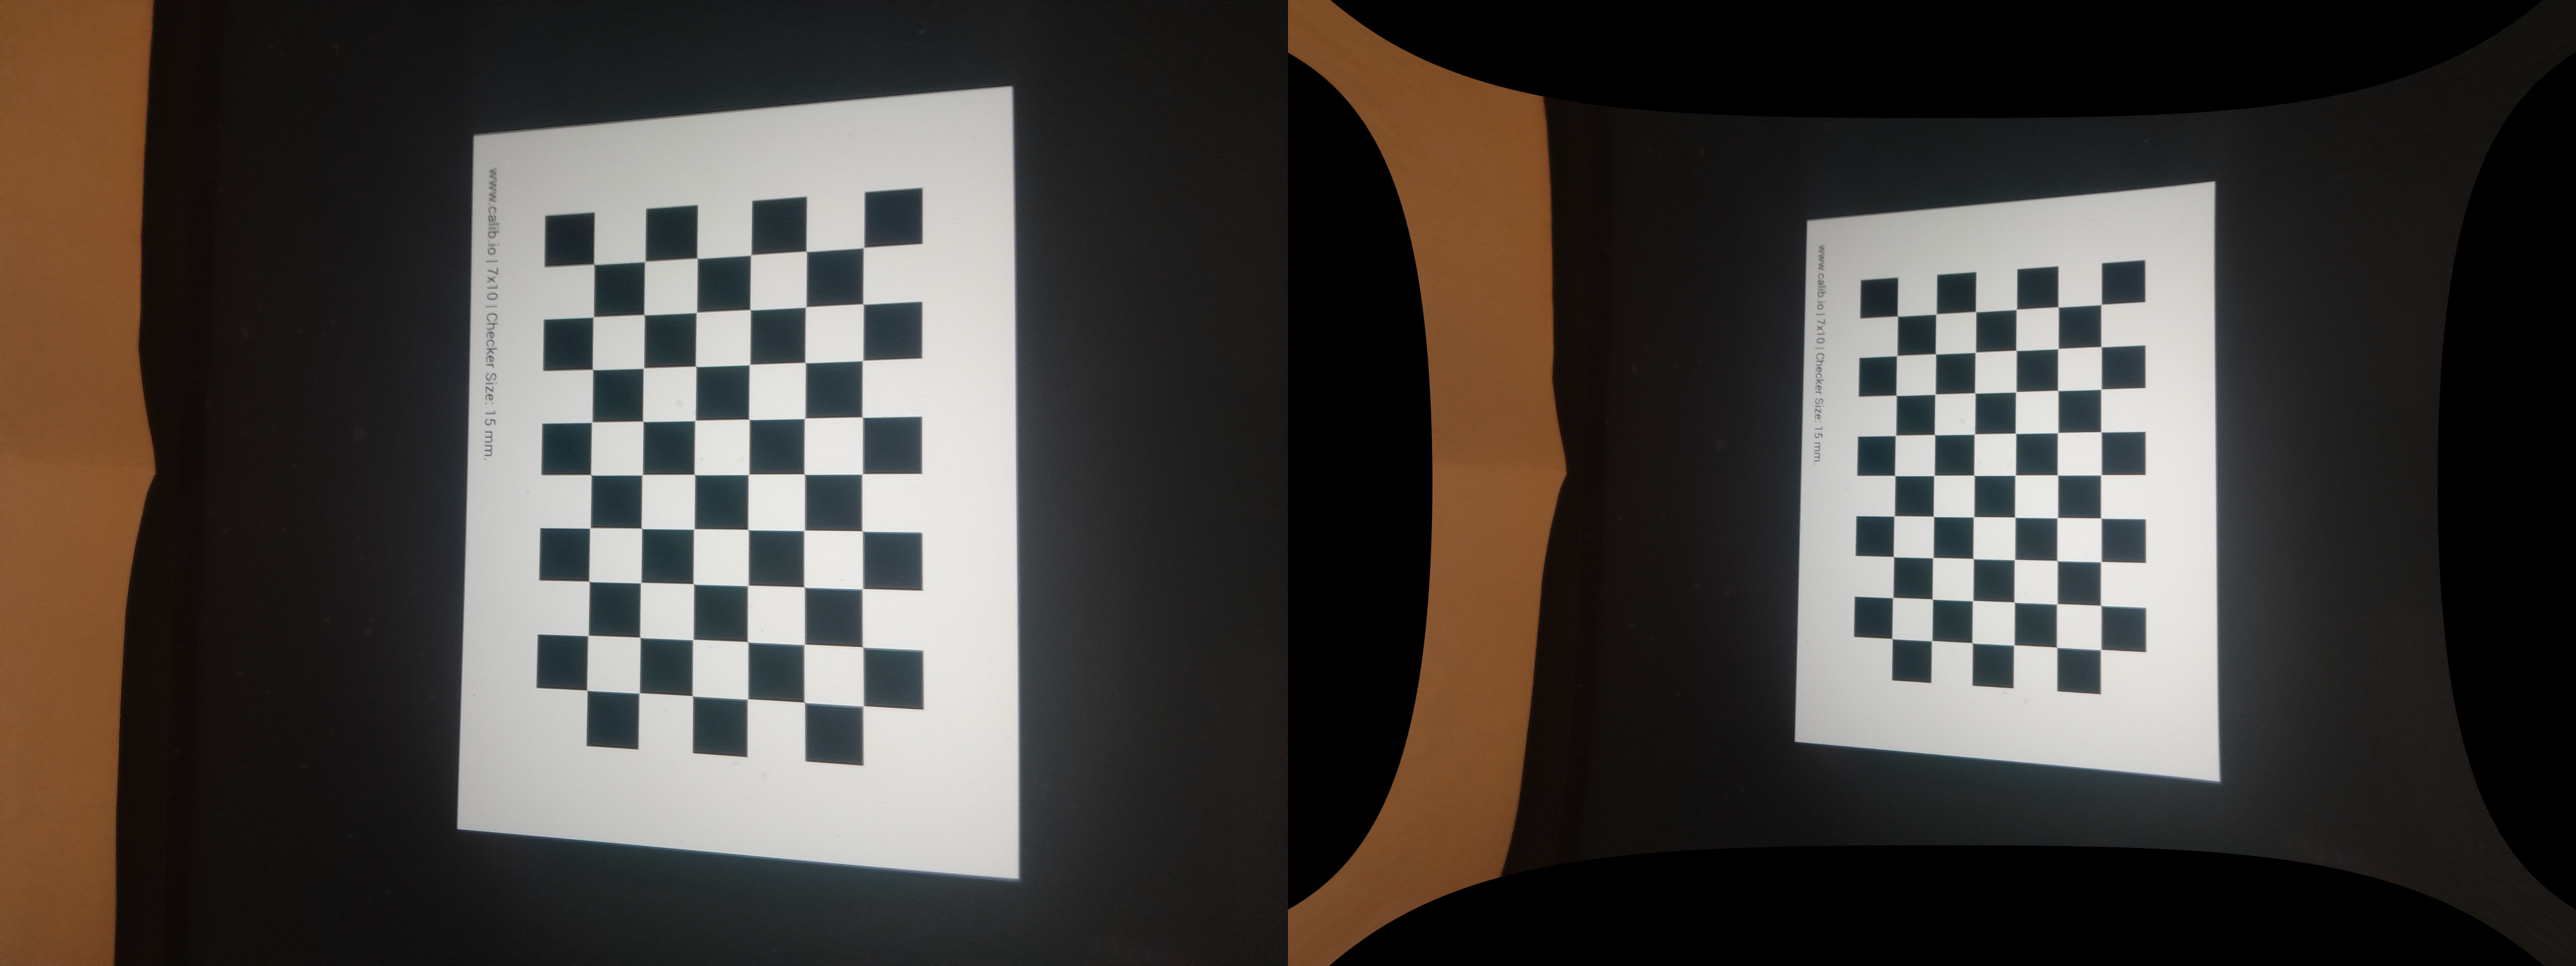
\includegraphics[width=0.95\textwidth]
    {figures/comparison.png}
    \caption{Comparaison d'une image avant et après correction
    de la distorsion.}
    \label{fig:undistortion}
\end{figure}

Cette comparaison illustre l'application pratique des paramètres
de calibration. Elle permet de visualiser les modifications
géométriques apportées à l'image par la correction de la distorsion.


\chapter{Conclusion générale}

Ce travail avait pour objectif de réaliser la calibration d'une
caméra de smartphone à partir de plusieurs images d'un damier
de dimensions connues, puis d'exploiter les paramètres estimés
pour déterminer les poses de la caméra et corriger la distorsion
des images.

L'expérience a été réalisée avec la caméra principale d'un
Samsung Galaxy A14 4G. Nous avons acquis 19 photographies
d'un damier comportant 9 colonnes et 6 lignes de coins
intérieurs. Après la détection et le raffinement subpixel des
points caractéristiques, 18 images ont été retenues pour
la calibration finale.

La calibration réalisée avec OpenCV a permis d'estimer la
matrice intrinsèque et les coefficients de distorsion de la
caméra. L'erreur quadratique moyenne de reprojection obtenue
est de 0,2678 pixel. La longueur focale physique estimée
est de 4,1951 mm, soit 0,0041951 m. Cette valeur est proche
de celle indiquée dans les métadonnées EXIF, qui est de
4,0 mm.

Nous avons ensuite estimé les poses de la caméra pour les
18 images à l'aide de la fonction \texttt{cv2.solvePnP()}.
La représentation tridimensionnelle obtenue permet de
visualiser les différentes positions et orientations de la
caméra par rapport au repère du damier.

L'évaluation des reprojections a donné une erreur moyenne
de 0,2146 pixel et une moyenne des RMSE individuels de
0,2484 pixel. Ces résultats montrent une bonne cohérence
entre les points détectés dans les images et leurs positions
reprojetées par le modèle de caméra.

Enfin, les paramètres estimés ont été utilisés pour corriger
la distorsion des images. La comparaison avant et après
correction a permis de visualiser l'effet de cette opération
sur la géométrie des images.

Cette expérience nous a permis de mettre en pratique les
principales étapes d'un processus de calibration : acquisition
des images, détection des points caractéristiques, estimation
des paramètres de la caméra, estimation des poses, évaluation
par reprojection et correction de la distorsion.

Certaines limites expérimentales doivent néanmoins être
prises en compte. Le damier ayant été affiché sur un écran
plutôt qu'imprimé, la mesure de la taille des carrés et la
planéité du support peuvent introduire des incertitudes.
De plus, les dimensions physiques du capteur utilisées pour
estimer la longueur focale sont des valeurs approximatives.
Ces éléments peuvent influencer la précision des résultats,
notamment leur interprétation en unités physiques.

En perspective, cette étude pourrait être améliorée en
utilisant un damier imprimé avec des dimensions précisément
mesurées, en réalisant davantage de prises de vue dans des
configurations variées et en comparant les résultats obtenus
avec d'autres méthodes de calibration.

\end{document}
